\section{Conception}
\noindent
Dans cette partie, nous allons présenter le diagramme de séquence correspondant à notre diagramme cas d'utilisation précédemment présentés dans les descriptions textuelles pour le deuxième Sprint.

\subsection{Diagramme de séquence détaillé}
\noindent
Nous avons regroupé les deux cas d'utilisation << Rechercher produits en Arabe traditionnel >> et << Rechercher produits en Arabe en dialecte Tunisien >> dans un seul diagramme de séquence présenté dans la figure ~\ref{fig:diagseqsprint2}.

\begin{figure}[H]
	\centering
	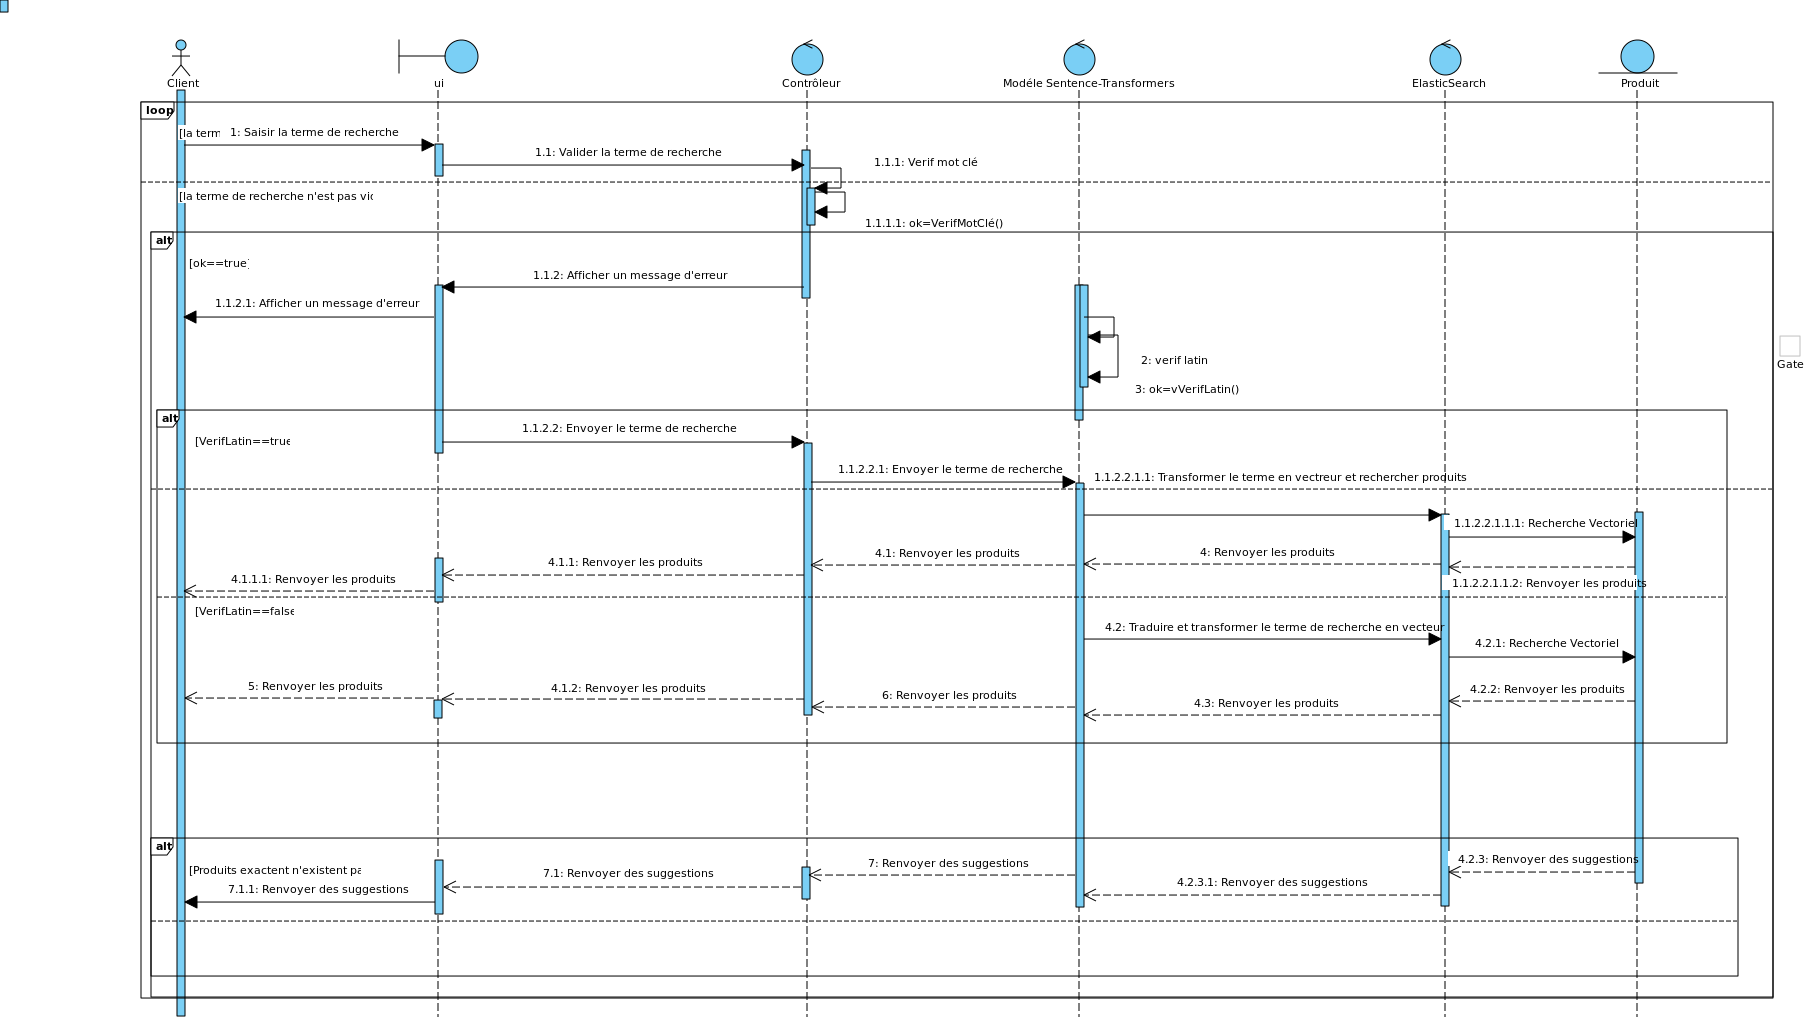
\includegraphics[width=1\textwidth]{logos/seqsprint2.png}
	\caption{Diagramme de séquence des cas d’utilisations « Rechercher produits en Arabe Traditionnel » et << Rechercher produits en Arabe en dialecte Tunisien >>}
	\label{fig:diagseqsprint2}
\end{figure}

\section{Réalisation}
\noindent
Cette partie est consacrée à la présentation des étapes nécessaires pour réaliser le travail nécessaire pour satisfaire notres cas d'utilisations, qui consiste à permettre le client ou le visiteur à rechercher notres produits en Arabe traditionnel et Arabe en dialecte tunisien tout en améliorant l'expérience de recherche en utilisant la traduction et la recherche vectorielle via Elasticsearch.

\newpage
\subsection{Les premières approches}
\noindent
Puisque notre modèle actuel n'est formé que sur les langues latines, nous avons eu l'idée de l'entraîner à la fois sur l'arabe tunisien et l'arabe traditionnel, mais un certain nombre de limitations nous empêchaient de le faire:

\begin{enumerate}
	\item Absence totale de jeux de données sur la langue arabe en dialecte Tunisien.
	\item Absence totale de jeux de données sur la langue Arabe Traditionnel.
	\item Le processus de l'entraînement nécessite une machine beaucoup plus puissante et une période de temps très longue afin de traiter correctement les 2 langues que nous avons citées.
\end{enumerate}

\noindent
Nous avons également testé avec le « Fine-Tuning » pour entraîner notre modéle, nous définissons ce processus comme suit: \\
\textit{Le << Fine-Tuning >> consiste à prendre un modèle d'apprentissage automatique pré-entraîné et à le former davantage sur un ensemble de données plus petit et ciblé. L'objectif du réglage fin est de conserver les capacités d'origine d'un modèle pré-entraîné tout en l'adaptant à des cas d'utilisation plus spécialisés.} \\ \citetitle{techtarget:finetuning} (\cite{techtarget:finetuning})

\noindent
Mais ce processus nécessitait un ensemble de données beaucoup plus volumineux que celui que nous avions préparé et prenait trop de temps, nous avons donc décidé d'adopter l'approche mentionnée ci-dessous.

\newpage
\subsection{Création de notre propre classe traducteur}
\noindent
Avec les limitations de l'approche << Fine-Tuning >> que nous avons mentionnée précédemment, nous avons décidé de créer notre propre traducteur qui va:
\begin{enumerate}
	\item Vérifier si le terme de recherche est en Arabe traditionnel, et le traduire en Français à partir de l'API Google Traduction.
	\item Vérifier si le terme de recherche est en Arabe en dialecte Tunisien à partir de notre propre dictionnaire des mots Tunisiens et leur equivalent en Français, si il n'y a pas d'équivalent exacte, il essaie de trouver l'équivalent en calculant un pourcentage, et s'il n'y a pas d'équivalent même après avoir calculé le pourcentage, le mot reste tel quel en supposant qu'il soit en Français
\end{enumerate}

\subsubsection{La création du dictionnaire}
\noindent
D'abord, nous commençons par préparer notre classe, que nous avons nommée << TunisianTranslator >> et initialiser un attribut privé, qui est notre dictionnaire. La figure ~\ref{fig:dictionary} montre le code nécessaire pour cette étape.

\begin{figure}[H]
	\centering
	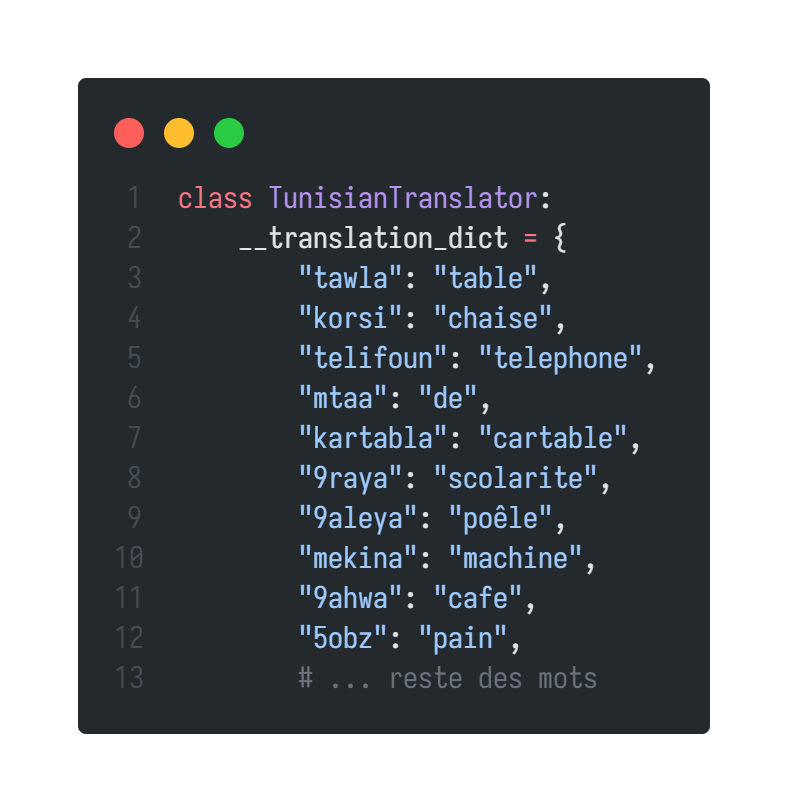
\includegraphics[width=0.6\textwidth]{logos/dictionary.png}
	\caption{Code d'initialisation de classe et du dictionnaire}
	\label{fig:dictionary}
\end{figure}

\noindent
Ensuite, nous continuons en définissant notre première méthode dans la classe qui est une méthode privée nommée \texttt{\_\_is\_latin}. Cette méthode est conçue pour vérifier si une chaîne donnée s contient uniquement des caractères des blocs Unicode Basic Latin et Latin-1 Supplement, elle renvoie True si tous les caractères de la chaîne << s >> se trouvent dans la plage Unicode U+0000 à U+00FF, ce qui correspond aux blocs Basic Latin et Latin-1 Supplement. Si un caractère se situe en dehors de cette plage, la méthode renvoie False.

\subsubsection{Analyse des expressions régulières}
\noindent
L'expression régulière utilisée dans notre méthode est :
\Large\[ [^{\backslash u0000-\backslash u00FF}] \]
\begin{itemize}
    \item \texttt{[...]}: Spécifie une classe de caractères, correspondant à n'importe quel caractère unique inclus entre parenthèses.
    \item \texttt{\^{}}: Entre parenthèses de classe de caractères, cela annule la classe, donc elle correspond à n'importe quel caractère \emph{non} répertorié entre parenthèses.
    \item \texttt{\textbackslash u0000-\textbackslash u00FF}: Définit une plage de caractères Unicode de \( U+0000 \) à \( U+00FF \), qui comprend à la fois les blocs Basic Latin et Latin-1 Supplement.
\end{itemize}

\newpage
\subsubsection{Logique de méthode}
\noindent
La méthode \texttt{re.search(r"[\textbackslash u0000-\textbackslash u00FF]", s)} recherche dans la chaîne \( s \), recherchant tout caractère en dehors de plage \( U+0000 \) jusqu'à \( U+00FF \):
\begin{itemize}
    \item Si un tel caractère est trouvé, \texttt{re.search} renvoie un objet de correspondance, qui est évalué à \texttt{True}.
    \item Si aucun caractère de ce type n'est trouvé (c'est-à-dire que tous les caractères sont dans la plage spécifiée), il renvoie \texttt{None}, qui est évalué à \texttt{False}.
\end{itemize}
L'utilisation de l'opérateur \texttt{not} inverse le résultat de \texttt{re.search}. Ainsi, la méthode renvoie \texttt{False} si des caractères se trouvent en dehors de la plage Unicode spécifiée, et \texttt{True} si tous les caractères s'y trouvent.

\noindent
La figure ~\ref{fig:islatin} illustre le code nécessaire pour cette méthode.

\begin{figure}[H]
	\centering
	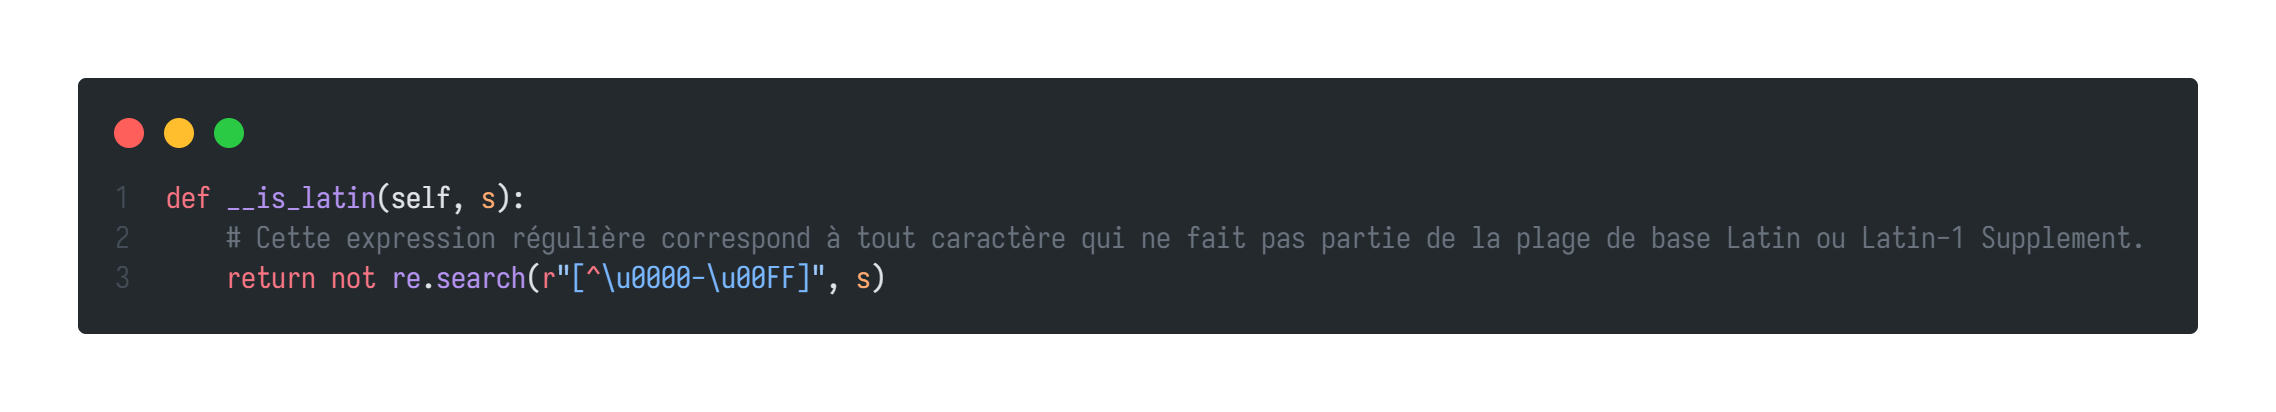
\includegraphics[width=1\textwidth]{logos/islatin.png}
	\caption{Code de méthode \_\_is\_latin}
	\label{fig:islatin}
\end{figure}